\subsection{Multiphase Bidirectional DC/DC Current Controller LM5170-Q1}
\indent The LM5170-q1\cite{TI_LM5170_User_Datasheet} controller is a high precision dual phase bidirectional converter applicated in automotive 48 Volts and 12Volts dual battery systems.
Depending on the Direction Signal DC/DC converter regulates the average current. 
The Regulated current through the DC/DC converter can be programmed by analog or Digital PWM inputs.

The LM5170-q1\cite{TI_LM5170_User_Datasheet} has a dedicated dual phase differential current sense amplifier to monitor the current flowing through the Dc/Dc converter, which can achieve $1\%$ current sense accuracy.
It has a Robust Gate driver to drive half the bridge. The Internal gate driver of the LM5170 has the capability of driving parallel MOSFET switches with a capacity of 500Watts. 
The synchronous diode emulation mode prevents the dc to dc converter from the negative currents and also enables the discontinuous mode of operation. This property enhances the DC/DC converter efficiency tremendously. The Controller can offer benefits of cycle-by-cycle current limitation, overVoltage protection at both low side and high side ports, Temperature protection and Mosfet failure so on...
\\
\indent An innovative average current mode control scheme maintains constant loop gain, allowing a single R-C network
to compensate both buck and boost conversion\cite[p .2]{TI_LM5170_User_Datasheet},\cite{TI_LM5170_EVM_User_Guide}. The oscillator is adjustable up to 500 kHz and can synchronize
to an external clock. Multiphase parallel operation is achieved by connecting two LM5170 controllers for 3-
or 4-phase operation, or by synchronizing multiple controllers to phase-shifted clocks for a higher number of
phases. A low state on the UVLO pin disables the LM5170 in a low current shutdown mode\cite{TI_LM5170_User_Datasheet}.

\subsubsection{Definition of IC LM5170 Operation Modes:}
\begin{itemize}
    \item \textbf{Shutdown Mode:} When the UVLO pin is < 1.25 V, VCC < 8 V, or default < 1.25 V, the LM5170 is in
    shutdown mode with all gate drivers in the low state, all internal logic reset, and the VINX pin disconnected
    from the VIN pin. When UVLO < 1.25 V, the IC draws < 20 µA through the VIN and VCC pins\cite{TI_LM5170_User_Datasheet}.
    \item \textbf{Initialization Mode:}  When the UVLO pin is > 1.5 V but < 2.5 V, VCC > 8.5 V, and nFAULT > 2 V, the LM5170
    establishes proper internal logic states and prepares for circuit operation\cite{TI_LM5170_User_Datasheet}.
    \item \textbf{Standby Mode:}  When the UVLO pin is > 2.5 V, VCC > 8.5 V, and nFAULT > 2 V, the LM5170 first
    performs fault detection for 2 to 3 ms. During this time, the external power MOSFETs are each checked for
    drain-to-source short-circuit conditions. If a fault is detected, the LM5170 returns to shutdown mode and is
    latched in shutdown until reset through the UVLO or VCC pins. If no failure is detected, the LM5170 is ready
    to operate. The circuit breaker MOSFETs are turned on and the oscillator and ramp generators are activated,
    but the four gate drive outputs remain off until the EN1 or EN2 initiate the power delivery mode\cite{TI_LM5170_User_Datasheet}.
    \item \textbf{Power Delivery Mode:}  When the UVLO pin > 2.5 V, VCC > 8.5 V, nFAULT > 2 V, EN1 or EN2 > 2 V, DIR
    is valid (> 2 V or < 1 V), and ISETA > 0 V, the SS capacitor is released and the LM5170 regulates the DC
    current at the level set at the ISETA pin\cite{TI_LM5170_User_Datasheet}.
\end{itemize}

\subsubsection{Bench setup and operation of the DC/DC Converter :}
Although LM5170 can perform full bridge operation, we need only the half-bridge with a full current rating for our application. Figure\ref{fig:LM5170_DC_DC_Converter_Operation_Setup} only the high side bridge is used for buck and boost operations. The Figure shows the typical setup to operate the DC/DC converter in the bidirectional power system environment. The combination of the Load on the High side is the Battery pack Top and on the Low side, the is Battery pack node.  A current Can flow from the High side to the low side or vice versa depending on the direction. The direction of the current flow depends on the BMS algorithm. A BMS algorithm decides which no needs to be balanced depending on batteries voltage difference. 
\begin{figure}[h]
	\centering
	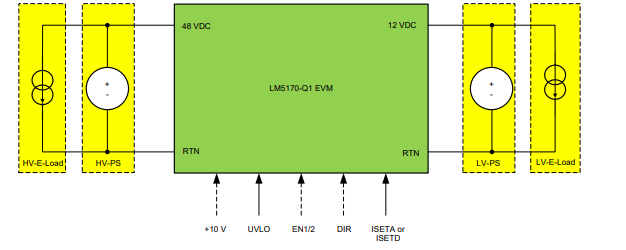
\includegraphics[width=1\textwidth]{Chap04/Figures/DC_DC_Converter_bench_setup.PNG}
	\caption{LM5170 DC/DC Converter Operation Setup \cite{TI_LM5170_BatteryTesting_Solution},\cite{TI_LM5170_EVM_User_Guide} }
	\label{fig:LM5170_DC_DC_Converter_Operation_Setup}
\end{figure}

\subsubsection{The operation of the DC converter is as follows (The Figure \ref{fig:LM5170_DC_DC_Converter_Operation_Setup}) :}
\begin{itemize}
    \item Connect the High side and Low side Battery pack nodes (Low or High side could be electronics loads also).
    \item Apply a voltage > 2.5 V and < 6 V  to the UVLO pin to release it from the shutdown mode.
    \item Select the EN1 or EN2 to enable the dc to dc converter output, for instance, EN1 is the output enable signal for phase1 and EN2 is the output enable signal for phase 2.
    \item Depending on the mode of operation Apply DIR pin voltages. Direction command input. Pulling DIR above 2 V sets the converter to buck mode, which commands the current to flow from the HV-Port to LV-Port. Pulling DIR below 1 V sets the converter to boost mode, which commands the current to flow from the LV-Port to HV-Port. If the DIR pin is left open, the LM5170 detects an invalid command and disables both phases with the MOSFET gate drivers in the low state\cite[p .5]{TI_LM5170_EVM_User_Guide}. 
    \item Use the ISETA signal to set the current.ISETA is the analog current programming pin. The inductor DC is proportional to the ISETA voltage. Use either ISETA or ISETD but not both for phase current programming. When ISETA is not used, connect a 100-pF to 0.1-µF capacitor from ISETA to AGND\cite[p .5]{TI_LM5170_EVM_User_Guide}.
    \item If the ISETD is used, The PWM current programming pin. The inductor DC level is proportional to the PWM duty cycle. Use either ISETA or ISETD but not both for phase current programming. When ISETD is not used, short ISETD to AGND \cite[p .6]{TI_LM5170_EVM_User_Guide}.
\end{itemize}
\subsubsection{Summary of the DC/DC Converter:}
\indent Although DC/DC Converter LM5170 is capable to use the dual phases, we have limited the DC/DC converter to the single phase according to the Type ii BMS DC/DC converter configuration. Depending on the user's need user can use ISETA or ISETD to setting the current flowing in the dc to dc converter. For Instance, if the user uses a microcontroller it is much more convenient to use the PWM, so the ISETD is a natural choice, If the user opts Central pc/ Labview application it is much better to use ISETA through some analog supply. Ultimately ISETD (PWM) converted to the Analog voltage to set the current.